\chapter{Espressioni regolari}
Diciamo che una parola è accettata oppure no in base allo stato in cui giungiamo alla
fine di questa parola (se sono in uno stato finale, allora si tratta di una parola accettata
dall'automa altrimenti no).
Un'espressione regolare è un modo dichiarativo per descrivere un linguaggio regolare.
Abbiamo diversi tipi di operazioni sui linguaggi:

\begin{itemize}
\item \textbf{Unione}: $L\cup M=\{w:w \in L oppure w \in M\}$
\item \textbf{Concatenazione}: $L.M=\{uv : u \in L e v \in M\}$
\item \textbf{Potenze}: 
	\begin{itemize}
	\item $L^{0}=\{\varepsilon\}$
	\item $L^{1}=L$   
	\item $L^{k}=L.L...L(k volte)$
	\end{itemize}
\item \textbf{Chiusura di Kleene}: $L^{\ast} = \bigcup_{i=0}^\infty L^{i}$
\end{itemize} 

Inoltre le espressioni regolari sono costruite utilizzando 

\begin{itemize}
\item un insieme di costanti di base:
	\begin{itemize}
	\item $\varepsilon$ per la stringa vuota
	\item $\emptyset$ per il linguaggio vuoto
	\item a,b,.. per i simboli $a,b,..\in \Sigma$
	\end{itemize}
\item collegati da operatori:
	\begin{itemize}
	\item $+$ per l'unione;
	\item $\cdot$ per la concatenazione;
	\item $\ast$ per la chiusura di Kleene;
	\end{itemize}
\end{itemize}

Esistono anche delle \textbf{regole di precedenza} degli operatori:
\begin{itemize}
\item[1]Chiusura di Kleene;
\item[2]Concatenazione;
\item[3]Unione.
\end{itemize}

\section{Equivalenza tra FA e RE}
DFA, NFA e $\varepsilon$\textrm{-NFA} sono tutti equivalenti.

\begin{figure}[h]
\centering 
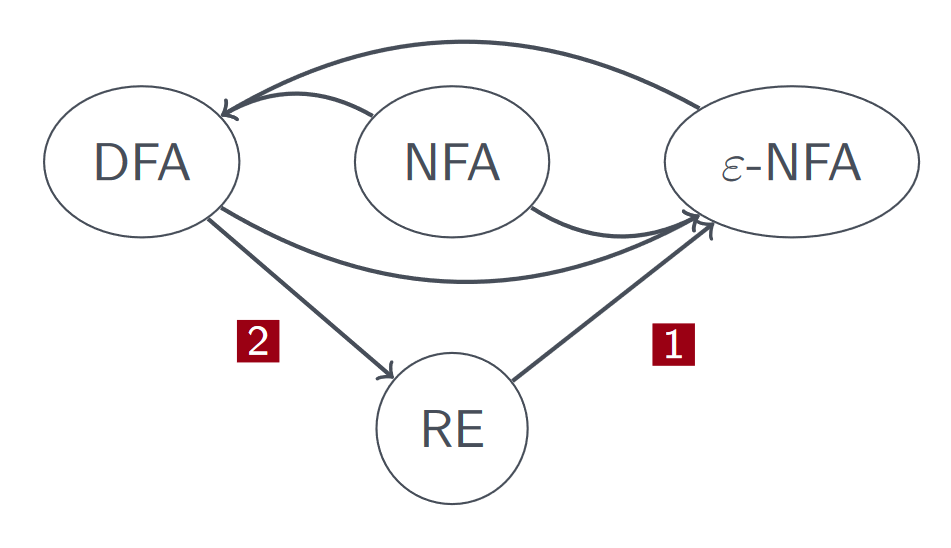
\includegraphics[scale=0.5]{Immagini/equivalenza3.png}
\end{figure}

Infatti 
\begin{itemize}
\item[1] Per ogni espressione regolare \textbf{R} esiste un $\varepsilon$\textrm{-
NFA}A, tale che L(A)=L(\textbf{R});
\item[2] Per ogni FA A possiamo costruire un'espressione regolare \textbf{R},
tale che L(\textbf{R})=L(A).
\end{itemize}

\section{Conversione per eliminazione di stati}
Quando uno stato \textbf{q} viene eliminato, i cammini che passano per q scompaiono.
Quindi si aggiungono nuove transizioni etichettate con espressioni regolari che 
rappresentano questi cammini eliminati. Alla fine otteniamo un'espressione regolare
che rappresenta tutti i cammini dallo stato iniziale ad uno stato finale, ovvero
\textbf{il linguaggio riconosciuto dall'automa}.






